\FILENAME

\chapter{Hardware}\label{hardware-description}

The Chameleon architecture consists of a set of standard cloud units
(SCUs), each of which is a single rack with 42 compute nodes, 4 storage
nodes attached to 128TB of local storage in configurable arrays, and an
OpenFlow compliant network switch. In addition to the homogeneous SCUs,
a variety of heterogeneous hardware types is available to experiment
with alternative technologies. The testbed also includes a shared
infrastructure with a persistent storage system accessible across the
testbed, a top-level network gateway to allow access to public networks,
and a set of management and provisioning servers to support user access,
control, monitoring and configuration of the testbed. Chameleon is
physically distributed between the Texas Advanced Computing Center
(TACC) and the University of Chicago (UC) through 100Gbps Internet2
links, to allow users to examine the effects of a distributed cloud.

\textbf{Hardware Summary}

\begin{longtable}[]{@{}ll@{}}
\toprule
Standard Cloud Units (SCUs) & Homogeneous Hardware Types\tabularnewline
Number of Nodes per Rack: & \vtop{\hbox{\strut 42 Compute
Nodes}\hbox{\strut 4 Storage Nodes}}\tabularnewline
Local Storage per homogeneous SCU: & 128TB (configurable)\tabularnewline
Network Switch: & OpenFlow Compliant\tabularnewline
TACC/UC Distributed Cloud & 100Gbps Internet2 links\tabularnewline
\bottomrule
\end{longtable}

\href{https://www.chameleoncloud.org/user/discovery/}{\emph{~}
\textbf{Detailed information in our Resource Discovery Portal}}


\paragraph{Standard Cloud Units}\label{standard-cloud-units}

The homogeneous~standard cloud unit is a self-contained rack with all
the components necessary to run a complete cloud infrastructure, and the
capability to combine with other units to form a larger experiment. The
rack consists of 42 Dell R630 servers; each with 24 cores delivered in
dual socket Intel Xeon E5-2670 v3 ``Haswell'' processors (each with 12
cores @ 2.3GHz) and 128 GiB of RAM. In addition to the compute servers,
each unit contains storage hosted in two FX2 chassis, each containing
two Dell FC430 servers attached to two Dell PowerEdge FD332 storage
blocks containing 16 2TB hard drives, for a total of 128TB of raw disk
storage per unit. These FC430 storage nodes contain dual socket Intel
Xeon E5-2650 v3 ``Haswell'' processors (each with 10 cores @ 2.3 GHz),
64 GiB of RAM, and can be combined across SCUs to create a Big Data
infrastructure with more than a PB of storage. Each node in the SCU
connects to a Dell switch at 10Gbps, with 40Gbps of bandwidth to the
core network from each SCU. The total system contains 12 SCUs (10 at
TACC and 2 at UC) for a total of 13,056 cores, 66 TiB of RAM, and 1.5PB
of configurable storage in the SCU subsystem.

\begin{figure}[htb]
\centering 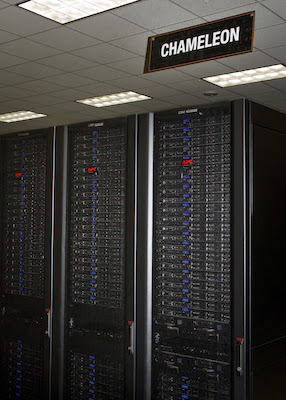
\includegraphics[width=0.5\columnwidth]{images/chameleon/Chameleon2.jpeg}
\caption{Chameleon Cloud Racks}
\end{figure}

\paragraph{Network}\label{network}

Networking is changing rapidly, and the network fabric is as much a part
of the research focus of Chameleon as the compute or storage. For the
Chameleon network, every switch in the research network is a fully
OpenFlow compliant programmable Dell S6000-ON switch. Each node connects
to this network at 10 Gbps, and each unit~uplinks with 40Gbps per rack
to the Chameleon core network. The core switches (Dell S6000-ON) are
connected by~40 Gbps Ethernet links, which connect to the backbone
100Gbps services at both UC and TACC.~A Fourteen Data Rate (FDR)
Infiniband network (56Gbps) is also deployed on one SCU to allow
exploration of alternate networks.


\paragraph{Shared Storage}\label{shared-storage}

While storage is dynamically provisioned to researchers to be used as an
experiment needs within the SCUs, Chameleon also provides a shared
storage system. The shared storage provides more than 3.6PB of raw disk
in the initial configuration, which is partitioned between a file system
and an object store that is persistent between experiments. The shared
storage is comprised of four Dell R630 servers with 128 GiB of RAM, four
MD3260 external drive arrays, and six MD3060e drive expansion chassis,
populated by 600 6TB near line SAS drives. The system also includes a
dozen PowerEdge R630 servers as management nodes to provide for login
access to the resource, data staging, system monitoring, and hosting
various OpenStack services.


\paragraph{Heterogeneous Compute
Hardware}\label{heterogeneous-compute-hardware}

The heterogeneous hardware includes various technologies: GPU and FPGA
accelerators, SSD and NVMe storage, low-power ARM, Atom, and Xeon
systems-on-a-chip. With the exception of the low-power
systems-on-a-chip, each of the additional nodes is a Dell PowerEdge R730
server with the same CPUs as the R630 servers in our SCUs.

The two storage hierarchy nodes have been designed to enable experiments
using multiple layers of caching: they are configured with 512 GiB of
memory, two Intel P3700 NVMe of 2~TB each, four Intel S3610 SSDs of 1.6
TB each, and four 15K SAS HDDs of 600 GB each.

The GPU offering consists of two K80 GPU nodes, two M40 GPU nodes,
sixteen P100 GPU nodes. These nodes target experiments using
accelerators to improve the performance of some algorithms, experiments
with new visualization systems, and deep machine learning. Each K80 GPU
node is upgraded with an NVIDIA Tesla K80 accelerator, consisting of two
GK210 chips with 2496 cores each (4992 cores in total) and 24 GiB of
GDDR5 memory. Each M40 node is upgraded with an NVIDIA Tesla M40
accelerator, consisting of a GM200 chip with 3072 cores and 12 GiB of
GDDR5 memory. The P100 nodes have two GPU cards installed each,
providing 32 P100 GPUs in total. The P100 GPUs utilize GP100 chips
providing 3584 cores, with 16 GiB GDDR5 RAM in each card.~In order to
make it easy for users to get started with the GPU nodes, we have
developed a~\href{https://www.chameleoncloud.org/appliances/21/}{CUDA
appliance} that includes NVIDIA drivers as well as the CUDA framework.

\begin{longtable}[]{@{}llllll@{}}
\toprule
GPU & Chip & Cores per GPU & RAM per GPU & GPU per node & \# of
nodes\tabularnewline
Tesla K80 & GK 210 & 2496 x 2 & 24 GiB GDDR5 & 1 & 2\tabularnewline
Tesla M40 & GM 200 & 3072 & 12 GiB GDDR5 & 1 & 2\tabularnewline
Tesla P100 & GP100 & 3584 & 16 GiB GDDR5 & 2 & 16\tabularnewline
\bottomrule
\end{longtable}

The four FPGA nodes have a~Nallatech 385A board with an Altera Arria 10
1150 GX FPGA (up to 1.5 TFlops), 8 GiB DDR3 on-card memory, and dual
QSFP 10/40 GbE support. The Chameleon
\href{https://www.chameleoncloud.org/docs/bare-metal-user-guide/fpga/}{FPGA
User Guide}~provides details for conducting experiments on this
hardware.

The low-power systems are comprised of 8 low power Xeon servers (HP
ProLiant m710p with one 4-core Intel Xeon E3-1284L v4 processor), 8 Atom
servers (HP ProLiant m300 with one 8-core Intel Avoton-based System on a
Chip), and 24 ARM servers (HP ProLiant m400 with one 8-core AppliedMicro
X-gene System on a Chip). These are all delivered in a single HP
Moonshot 1500 chassis.

For more information on how you can reserve these nodes, see the
\href{https://www.chameleoncloud.org/docs/bare-metal-user-guide/\#heterogeneous_hardware}{heterogeneous
hardware section} of the bare metal user's guide.


\paragraph{Live updates}
You can browse detailed information about the resources
offered~for bare metal reconfiguration in our
\href{https://www.chameleoncloud.org/user/discovery/}{Resource Discovery
Portal}.
